\documentclass[12pt]{article}
\usepackage{pgfplots}
\usepackage[utf8]{inputenc}
\usepackage[T1]{fontenc}
\usepackage{lmodern}
\usepackage{geometry}
\usepackage{tikz}
\pgfplotsset{compat=1.18}
\geometry{
  a4paper,
  top=0.6in,
  left=0.6in,
  right=0.6in,
  bottom=0.8in,
}
\usepackage{longtable}
\usepackage{amsmath}
\usepackage{graphicx}
\usepackage{hyperref}
\usepackage{enumitem}
\usepackage{titlesec}

\setlength\parindent{0pt}

\titleformat{\section}{\large\bfseries}{\thesection}{1em}{}
\titleformat{\subsection}{\normalsize\bfseries}{\thesubsection}{1em}{}

\begin{document}

\begin{titlepage}
  \centering
  \vspace*{1cm}
  \textbf{\Large Capstone Project} \\
  \vspace{0.5cm}
  \textbf{Ayvu: Read research papers for fun} \\
  \vspace{1cm}
  \today \\
  \vspace{1cm}
  \textbf{Author: Santhosh} \\
  \vfill
\end{titlepage}

\tableofcontents
\newpage

\section{Team Contract}
% Defining responsibilities and communication protocols
This project is undertaken by a solo developer, eliminating the need for a formal team contract. However, to maintain structure and accountability, the following self-imposed guidelines are established:

\begin{itemize}
  \item \textbf{Responsibilities}: The developer is responsible for all aspects of the project, including conception, design, implementation, testing, and deployment.
  \item \textbf{Communication}: Weekly progress reports will be maintained in a personal log and submitted as required. Feedback from the instructor will be actively sought via email or course platforms.
  \item \textbf{Schedule}: Weekly milestones will be set every Sunday, with dedicated work hours of 10–15 hours per week, including 2 hours for planning and reflection.
  \item \textbf{Decision-Making}: All decisions will be documented with rationale to ensure clarity and traceability.
  \item \textbf{Conflict Resolution}: As a solo project, conflicts are internal. Any challenges will be addressed by consulting course resources, instructor guidance, or external references (e.g., documentation, forums).
\end{itemize}

\section{Concept of Operations (CONOPS)}
% Outlining the purpose, scope, and features of the proposed solution
\subsection{Purpose}
Ayvu is a website that aims to simplify the process of accessing, reading, and understanding academic papers from arXiv (at least for the MVP). By integrating PDF parsing, cloud storage, and AI-driven features, the platform will provide an intuitive interface for researchers, students, and professionals to engage with complex research content efficiently.

\subsection{Product Scope}
The software addresses the challenge of navigating dense academic papers by offering a streamlined platform to fetch, parse, store, and interact with research papers. The target audience includes:
\begin{itemize}
  \item \textbf{Researchers and Academics}: Seeking efficient ways to read and annotate papers.
  \item \textbf{Students}: Learning to engage with technical literature.
  \item \textbf{Professionals}: Exploring research in their fields.
\end{itemize}
The platform is relevant in an era where open-access repositories like arXiv are widely used, but the complexity of research papers can be a barrier to comprehension. By leveraging AI and user-friendly design, the solution enhances accessibility and learning.

\subsection{Product Description}
The website will allow users to:
\begin{itemize}
  \item Input an arXiv link to fetch and parse a research paper into a readable markdown format.
  \item Store papers and annotations in a dedicated Google Drive folder.
  \item Interact with content via AI-driven features, such as highlighting key sections, asking questions, and learning unfamiliar concepts.
  \item Access a clean, responsive interface for reading and note-taking.
\end{itemize}
Key features include:
\begin{itemize}
  \item \textbf{Paper Parsing}: Convert PDFs to markdown using algorithmic approaches or LaTeX source.
  \item \textbf{Cloud Storage}: Seamless integration with Google Drive for storing papers and notes.
  \item \textbf{AI Assistance}: LLM-powered tools for summarizing, explaining concepts, and answering queries.
  \item \textbf{User Interface}: A modern, responsive front-end for intuitive navigation.
\end{itemize}

\section{Domain Model}
% Describing entities and relationships in the problem domain
The domain model captures the core entities and their relationships within the research paper reading ecosystem:

\begin{itemize}
  \item \textbf{User}: Represents an individual using the platform, identified by their Google account. Users can upload arXiv links, read parsed papers, and interact with AI features.
  \item \textbf{Research Paper}: A document fetched from arXiv, containing metadata (e.g., title, authors, abstract) and content (PDF or LaTeX). It is parsed into markdown for display.
  \item \textbf{Google Drive Folder}: A dedicated storage space for each user, containing raw PDFs, parsed markdown files, and user notes.
  \item \textbf{Note}: Annotations or comments created by the user, linked to a specific paper or section.
  \item \textbf{AI Assistant}: An LLM-based component that processes user queries, highlights key sections, and explains concepts.
\end{itemize}

\textbf{Relationships}:
\begin{itemize}
  \item A \textbf{User} has one \textbf{Google Drive Folder}.
  \item A \textbf{Google Drive Folder} contains multiple \textbf{Research Papers} and \textbf{Notes}.
  \item A \textbf{Research Paper} is associated with multiple \textbf{Notes} and interacts with the \textbf{AI Assistant}.
  \item The \textbf{AI Assistant} processes \textbf{Research Papers} and \textbf{User} queries.
\end{itemize}

\textbf{Rationale}: The domain model focuses on the user's interaction with research papers, emphasizing storage and AI-driven comprehension. It simplifies the complexity of academic content by breaking it into manageable entities (papers, notes) and leveraging external services (Google Drive, AI) for scalability. This is visualized in figure \ref{fig:domainModel}.

\begin{figure}
  \centering
  \includegraphics[width=0.75\linewidth]{EntityRelationshipDiagram.png}
  \caption{Domain Model}
  \label{fig:domainModel}
\end{figure}

\section{Toolset Selection}
% Specifying tools and their rationale
The following tools are selected for development, testing, and deployment:

\begin{itemize}
  \item \textbf{Deno (Backend Runtime)}: A secure, lightweight runtime for TypeScript, suitable for edge environments due to its minimal dependencies and built-in TypeScript support.
  \item \textbf{Visual Studio Code (IDE)}: A versatile IDE with extensions for TypeScript, Svelte, and Git integration, supporting efficient development and debugging.
  \item \textbf{Vitest (Test Framework)}: A fast, Deno-compatible testing framework for unit and integration tests, ensuring robust backend and front-end testing.
  \item \textbf{Git/GitHub (Source Control)}: Git for version control, with GitHub as the repository for code management and CI/CD integration.
  \item \textbf{Vercel (Hosting)}: A free hosting platform optimized for SvelteKit, offering easy deployment and scalability.
  \item \textbf{Google Drive API}: Facilitates storage and retrieval of papers and notes, leveraging users' existing Google accounts.
\end{itemize}

\textbf{Rationale}: Deno is chosen for its edge compatibility and TypeScript support, aligning with the backend's requirements. VS Code provides a unified development environment. Vitest ensures efficient testing, while Git/GitHub supports version control and collaboration. Vercel is selected for its seamless SvelteKit integration, and Google Drive API offers reliable, user-owned storage.

\section{Programming Languages}
% Listing programming languages and their rationale
\begin{itemize}
  \item \textbf{TypeScript}: Used for backend development with Deno and front-end logic in SvelteKit. Its static typing enhances code reliability and maintainability.
  \item \textbf{Svelte (SvelteKit)}: A JavaScript framework for building the reactive front-end, chosen for its simplicity and performance.
  \item \textbf{SCSS}: For styling the front-end, offering modular and maintainable CSS with variables and nesting.
\end{itemize}

\textbf{Rationale}: TypeScript ensures type safety across the stack, reducing errors. SvelteKit provides a modern framework for fast, component-based UI development. SCSS enhances styling flexibility while keeping the codebase organized.

\section*{Participation}

\textbf{Standard of Work}:I will validate that the work is completed to a high-quality standard by committing to a minimum code coverage threshold of at least 90\% for unit tests, with a target code coverage threshold of 100\%. All major functional requirements, such as PDF parsing, Google Drive integration, AI-assisted features, and the SvelteKit frontend, will be validated with integration or end-to-end tests.
The application will also be accessibility tested using tools like Lighthouse or Wave to verify that there are no automated accessibility issues. Keyboard navigation and responsive design testing will be performed. All deliverables and project artifacts, such as the CONOPS, domain model, architecture diagrams, and documentation, will be completed in accordance with the necessary quality levels. \\

\textbf{Strategies to Achieve Standard of Work}: I will leverage my knowledge from previous courses and any relevant work experience to achieve high-quality outcomes consistent with the standard of work described above. This includes following an agile-like approach incorporating SCRUM, Kanban, and DevOps best practices for development, such as continuous integration with GitHub Actions and deployment to Vercel. \\

\textbf{Role Definition}: I will assume all responsibilities conventionally performed by a development team as part of the development process. I will formulate requirements, design the backend parsing logic, integrate storage and AI components, develop the frontend UI, test all parts, and perform project management functions. \\

\textbf{Deadlines}: I will submit all deliverables by the applicable deadlines; when possible, I will aim to submit deliverables in advance of the deadlines.

\section{Completion of work}

To complete work with a high quality and on time, work must be organized and structured.
\begin{itemize}
  \item Every Monday, I will perform backlog refinement. I will select the work for the week, create new tickets for tasks like backend parsing implementation or AI feature integration, update existing tickets as needed, and review the goals I have set.
  \item Every Monday, I will start a document for the assignment of the week to add to over the course of the week, including updates on domain model evolution or toolset adjustments.
  \item I will use a Kanban board with epics to organize tasks. Coding tasks (e.g., Deno backend development, SvelteKit UI components) and writing tasks (e.g., progress reports) alike will be listed here.
  \item I will create tickets to formalize the design before I start implementing its software, such as detailing the PDF parsing algorithm or Google Drive API flows.
  \item Every Monday, Wednesday, and Friday, I will review the board, create new tickets, identify areas in which I lack knowledge (e.g., mupdf.js usage or LLM integration) and need to learn about, and reprioritize the selected work for the week.
  \item Every Saturday, I will put technical work aside and focus on the written assignment for the week if I feel that not enough progress has been made on it in comparison to the technical tasks.
  \item I will use git branches to prototype new features, such as testing LaTeX-to-Markdown conversion. For each new feature, I will create unit tests with Vitest and GitHub Actions and require that they all pass before the new feature can be merged.
  \item I will maintain documentation. Comments in the code, usage instructions for the website, and rationale for choices like edge environment compatibility are important.
\end{itemize}

\section{Roadblock Mitigation}
Spending too much time on something that I am blocked on is counter productive. It is important to identify such tasks early. Backlog refinements is a good time to review this. I must balance working on easier tasks first and making sure that I do not run out of time to work on the blocked item.

Some possible ways I could resolve a roadblock is dedicating time to do research and training (e.g., on algorithmic PDF parsing techniques or Google Drive API permissions), identifying technical tasks that must be completed before the roadblock can be cleared (e.g., setting up Deno environment before parsing logic), and reaching out for help from the professor or experts online (e.g., forums for SvelteKit or AI integration issues).

\section{Team Consequences}
Not applicable, as this is a solo project.

\section{Personal Accountability Statements}
I will observe the PSU Code of Conduct and PSU Academic Integrity. I will complete this project to the best of my ability and in accordance with proper academic standards.
\begin{itemize}
  \item PSU Code of Conduct: https://studentaffairs.psu.edu/support-safety-conduct/student-conduct/code-conduct
  \item PSU Academic Integrity: hUps://ed.psu.edu/current-students/academic-integrity/ai-form Page
\end{itemize}

\section{Software Requirements}

The following table lists the initial formal software requirements for the \textit{Ayvu} website, derived from the project's concept of operations (CONOPS), product scope, and main features. These requirements focus on the core functionalities related to user authentication, paper fetching, parsing, storage, reading, and AI-assisted interactions. They are expressed in the IEEE 29148 format using ``The system shall...'' statements. Approximately 15 functional requirements have been identified to cover the essential aspects of the MVP.

\begin{table}[htbp]
  \centering
  \caption{Software Requirements}
  \label{tab:software-requirements}
  \begin{tabular}{|c|p{15cm}|}
    \hline
    \textbf{ID \#} & \textbf{Description} \\
    \hline
    RPR-1 & The system shall allow users to sign up and sign in exclusively via Google OAuth. \\
    \hline
    RPR-2 & The system shall request and obtain permissions from the user to access their Google Drive for storage operations. \\
    \hline
    RPR-3 & The system shall create a dedicated folder (e.g., ``Ayvu'') in the user's Google Drive upon initial sign-in. \\
    \hline
    RPR-4 & The system shall allow users to input an arXiv paper URL or ID to fetch the paper. \\
    \hline
    RPR-5 & The system shall fetch metadata (title, authors, abstract, and other relevant details) from the arXiv API. \\
    \hline
    RPR-6 & The system shall download the PDF version of the research paper from arXiv. \\
    \hline
    RPR-7 & The system shall parse the downloaded PDF into a readable markdown format using algorithmic methods or LaTeX source as a fallback. \\
    \hline
    RPR-8 & The system shall store the raw PDF, parsed markdown, and metadata in the user's dedicated Google Drive folder. \\
    \hline
    RPR-9 & The system shall provide a responsive web interface for viewing the parsed markdown content of the paper. \\
    \hline
    RPR-10 & The system shall allow users to add notes and highlights to specific sections of the displayed paper content. \\
    \hline
    RPR-11 & The system shall save user-added notes and highlights as separate files or annotations in the Google Drive folder associated with the paper. \\
    \hline
    RPR-12 & The system shall integrate an AI assistant to answer user questions about the paper's content. \\
    \hline
    RPR-13 & The system shall allow users to select text in the reading interface and request AI explanations for unfamiliar terms or concepts. \\
    \hline
    RPR-14 & The system shall use the AI assistant to highlight key sections or concepts in the paper upon user request. \\
    \hline
    RPR-15 & The system shall provide AI-generated suggestions for related learning resources or summaries to enhance user comprehension. \\
    \hline
  \end{tabular}
\end{table}

\section{Product Backlog}

The product backlog for Ayvu is presented below. The backlog comprises functional and architectural requirements mapped to 15 User Stories, adhering to the IEEE 29148 format and the User Story template.

Each User Story is derived from the software requirements (Table \ref{tab:software-requirements}) and includes a title, priority, effort estimation (using Fibonacci sequence for story points), a description in the format:
\textbf{`As a <user>, I want <function> so that <benefit>`}
and acceptance criteria in the Given-When-Then format. The requirements cover user authentication, paper fetching, parsing, storage, reading, and AI-assisted interactions, ensuring alignment with Ayvu's goal of simplifying academic paper comprehension while prioritizing user privacy and edge-friendly design.

\begin{longtable}{|c|p{15cm}|}
  \caption{Product Backlog for Ayvu}
  \label{tab:product-backlog} \\
  \hline
  \textbf{ID \#} & \textbf{User Story} \\
  \hline
  US-1 &
  \textbf{Title:} Sign in with Google \newline
  \textbf{Priority:} High \newline
  \textbf{Story Point Estimation:} 3 \newline
  \textbf{User Story:} As a user, I want to sign in using Google OAuth so that I can securely access Ayvu without creating a separate account. \newline
  \textbf{Acceptance Criteria:} Given a user is on the login page, when they select ``Sign in with Google'' and authenticate, then they are logged into Ayvu with their Google ID. \\
  \hline

  US-2 &
  \textbf{Title:} Grant Drive Permissions \newline
  \textbf{Priority:} High \newline
  \textbf{Story Point Estimation:} 3 \newline
  \textbf{User Story:} As a user, I want to grant Google Drive permissions so that Ayvu can store my papers and notes securely. \newline
  \textbf{Acceptance Criteria:} Given a user is signing in for the first time, when they authenticate via Google OAuth, then Ayvu requests and receives Drive permissions, and a ``Ayvu'' folder is created. \\

  \hline
  US-3 &
  \textbf{Title:} Create Drive Folder \newline
  \textbf{Priority:} High \newline
  \textbf{Story Point Estimation:} 2 \newline
  \textbf{User Story:} As a user, I want Ayvu to create a dedicated folder in my Google Drive so that all my papers and notes are organized. \newline
  \textbf{Acceptance Criteria:} Given a user has granted Drive permissions, when they sign in, then a folder named ``Ayvu'' is created in their Google Drive. \\

  \hline
  US-4 &
  \textbf{Title:} Input arXiv Paper \newline
  \textbf{Priority:} Medium \newline
  \textbf{Story Point Estimation:} 3 \newline
  \textbf{User Story:} As a user, I want to input an arXiv URL or ID so that I can fetch a research paper for reading. \newline
  \textbf{Acceptance Criteria:} Given a user is logged in, when they enter a valid arXiv URL or ID and submit, then the system fetches the paper's metadata and PDF. \\

  \hline
  US-5 &
  \textbf{Title:} Fetch Paper Metadata \newline
  \textbf{Priority:} High \newline
  \textbf{Story Point Estimation:} 3 \newline
  \textbf{User Story:} As a user, I want Ayvu to fetch a paper's metadata so that I can review its details before reading. \newline
  \textbf{Acceptance Criteria:} Given a valid arXiv URL or ID is submitted, when the system queries the arXiv API, then it retrieves and displays the title, authors, and abstract. \\

  \hline
  US-6 &
  \textbf{Title:} Download Paper PDF \newline
  \textbf{Priority:} High \newline
  \textbf{Story Point Estimation:} 3 \newline
  \textbf{User Story:} As a user, I want Ayvu to download the paper's PDF so that I can access its full content. \newline
  \textbf{Acceptance Criteria:} Given a valid arXiv URL or ID, when the system processes the request, then the PDF is downloaded and stored in the user's Google Drive. \\

  \hline
  US-7 &
  \textbf{Title:} Parse PDF to Markdown \newline
  \textbf{Priority:} High \newline
  \textbf{Story Point Estimation:} 8 \newline
  \textbf{User Story:} As a user, I want the paper's PDF to be converted to markdown so that I can read it easily on any device. \newline
  \textbf{Acceptance Criteria:} Given a downloaded PDF, when the system applies parsing algorithms or LaTeX fallback, then the content is converted to markdown and stored in Google Drive. \\

  \hline
  US-8 &
  \textbf{Title:} Store Files in Drive \newline
  \textbf{Priority:} High \newline
  \textbf{Story Point Estimation:} 3 \newline
  \textbf{User Story:} As a user, I want all paper files to be stored in my Google Drive so that I retain control over my data. \newline
  \textbf{Acceptance Criteria:} Given a fetched paper, when the PDF, markdown, and metadata are generated, then they are saved in the ``Ayvu'' folder. \\

  \hline
  US-9 &
  \textbf{Title:} View Markdown Content \newline
  \textbf{Priority:} High \newline
  \textbf{Story Point Estimation:} 5 \newline
  \textbf{User Story:} As a user, I want to view the parsed markdown content in a clean interface so that I can read the paper comfortably. \newline
  \textbf{Acceptance Criteria:} Given a parsed markdown file, when the user selects the paper, then the content is displayed in a responsive web interface. \\

  \hline
  US-10 &
  \textbf{Title:} Add Notes and Highlights \newline
  \textbf{Priority:} Medium \newline
  \textbf{Story Point Estimation:} 5 \newline
  \textbf{User Story:} As a user, I want to add notes and highlights to paper sections so that I can track my thoughts and key points. \newline
  \textbf{Acceptance Criteria:} Given a user is viewing a paper, when they highlight text or add a note, then the annotations are saved and linked to the paper. \\

  \hline
  US-11 &
  \textbf{Title:} Save Annotations \newline
  \textbf{Priority:} Medium \newline
  \textbf{Story Point Estimation:} 3 \newline
  \textbf{User Story:} As a user, I want my notes and highlights to be saved in Google Drive so that I can access them later. \newline
  \textbf{Acceptance Criteria:} Given a user adds notes or highlights, when they save their changes, then the annotations are stored in the ``Ayvu'' folder. \\

  \hline
  US-12 &
  \textbf{Title:} Query Paper Content \newline
  \textbf{Priority:} Medium \newline
  \textbf{Story Point Estimation:} 5 \newline
  \textbf{User Story:} As a user, I want to ask questions about the paper's content so that I can clarify concepts. \newline
  \textbf{Acceptance Criteria:} Given a user is viewing a paper, when they submit a question via the AI interface, then the AI provides a relevant answer based on the paper's content. \\

  \hline
  US-13 &
  \textbf{Title:} Explain Selected Text \newline
  \textbf{Priority:} Medium \newline
  \textbf{Story Point Estimation:} 5 \newline
  \textbf{User Story:} As a user, I want to select text and request AI explanations so that I can understand unfamiliar terms or concepts. \newline
  \textbf{Acceptance Criteria:} Given a user selects text in the paper, when they request an explanation, then the AI provides a clear explanation of the selected content. \\

  \hline
  US-14 &
  \textbf{Title:} Highlight Key Sections \newline
  \textbf{Priority:} Medium \newline
  \textbf{Story Point Estimation:} 5 \newline
  \textbf{User Story:} As a user, I want the AI to highlight key sections or concepts so that I can focus on important parts of the paper. \newline
  \textbf{Acceptance Criteria:} Given a user is viewing a paper, when they request key section highlights, then the AI identifies and highlights critical parts in the interface. \\

  \hline
  US-15 &
  \textbf{Title:} Suggest Learning Resources \newline
  \textbf{Priority:} Low \newline
  \textbf{Story Point Estimation:} 5 \newline
  \textbf{User Story:} As a user, I want AI-generated suggestions for related resources or summaries so that I can deepen my understanding. \newline
  \textbf{Acceptance Criteria:} Given a user is viewing a paper, when they request suggestions, then the AI provides relevant resources or summaries based on the paper's content. \\

  \hline
\end{longtable}

\section{Sprint Backlog}
\label{sec:sprint-backlog}

The Sprint Backlog for Ayvu is presented below. This backlog is a prioritized subset of the Product Backlog (Table \ref{tab:product-backlog}), focusing on foundational requirements critical to building the Minimum Viable Product (MVP) during the two-week sprint. The selected User Stories emphasize user authentication, Google Drive integration, and core paper fetching and parsing functionalities, as these are essential for enabling the basic workflow of the application. The prioritization considers dependencies (e.g., authentication and storage setup must precede paper fetching) and the criticality of features for the MVP, with effort estimations based on the Fibonacci sequence (1, 2, 3, 5, 8, 13). The Sprint Backlog is managed in a project management tool (e.g., GitLab), ensuring alignment with the agile development process.

The sprint backlog is built on Github Projects, which is linked to the GitHub repository for the project. The board has columns for Backlog, To Do, In Progress, In Review, and Done. Each user story is represented as a card on the board, with tasks broken down into smaller sub-tasks as needed. The board is reviewed and updated regularly to reflect the current status of each task. You can view the project board here: \url{https://github.com/users/ABSanthosh/projects/20/views/1}

\begin{longtable}{|c|p{16cm}|}
  \caption{Sprint Backlog for Ayvu (First Sprint)}
  \label{tab:sprint-backlog} \\
  \hline
  \textbf{ID \#} & \textbf{User Story} \\
  \hline
  US-1 &
  \textbf{Title:} Sign in with Google \newline
  \textbf{Priority:} High \newline
  \textbf{Estimation:} 3 \newline
  \textbf{User Story:} As a user, I want to sign in using Google OAuth so that I can securely access Ayvu without creating a separate account. \newline
  \textbf{Acceptance Criteria:} Given a user is on the login page, when they select ``Sign in with Google'' and authenticate, then they are logged into Ayvu with their Google ID. \\
  \hline
  US-2 &
  \textbf{Title:} Grant Drive Permissions \newline
  \textbf{Priority:} High \newline
  \textbf{Estimation:} 3 \newline
  \textbf{User Story:} As a user, I want to grant Google Drive permissions so that Ayvu can store my papers and notes securely. \newline
  \textbf{Acceptance Criteria:} Given a user is signing in for the first time, when they authenticate via Google OAuth, then Ayvu requests and receives Drive permissions, and a ``Ayvu'' folder is created. \\
  \hline
  US-3 &
  \textbf{Title:} Create Drive Folder \newline
  \textbf{Priority:} High \newline
  \textbf{Estimation:} 2 \newline
  \textbf{User Story:} As a user, I want Ayvu to create a dedicated folder in my Google Drive so that all my papers and notes are organized. \newline
  \textbf{Acceptance Criteria:} Given a user has granted Drive permissions, when they sign in, then a folder named ``Ayvu'' is created in their Google Drive. \\
  \hline
  US-5 &
  \textbf{Title:} Fetch Paper Metadata \newline
  \textbf{Priority:} High \newline
  \textbf{Estimation:} 3 \newline
  \textbf{User Story:} As a user, I want Ayvu to fetch a paper's metadata so that I can review its details before reading. \newline
  \textbf{Acceptance Criteria:} Given a valid arXiv URL or ID is submitted, when the system queries the arXiv API, then it retrieves and displays the title, authors, and abstract. \\
  \hline
  US-6 &
  \textbf{Title:} Download Paper PDF \newline
  \textbf{Priority:} High \newline
  \textbf{Estimation:} 3 \newline
  \textbf{User Story:} As a user, I want Ayvu to download the paper's PDF so that I can access its full content. \newline
  \textbf{Acceptance Criteria:} Given a valid arXiv URL or ID, when the system processes the request, then the PDF is downloaded and stored in the user's Google Drive. \\
  \hline
  US-8 &
  \textbf{Title:} Store Files in Drive \newline
  \textbf{Priority:} High \newline
  \textbf{Estimation:} 3 \newline
  \textbf{User Story:} As a user, I want all paper files to be stored in my Google Drive so that I retain control over my data. \newline
  \textbf{Acceptance Criteria:} Given a fetched paper, when the PDF, markdown, and metadata are generated, then they are saved in the ``Ayvu'' folder. \\
  \hline
\end{longtable}

\subsection{Prioritization and Estimation Rationale}
The Sprint Backlog includes User Stories US-1, US-2, US-3, US-5, US-6, and US-8, selected for their foundational role in enabling Ayvu's core functionality. US-1 (Sign in with Google) and US-2 (Grant Drive Permissions) are prerequisites for US-3 (Create Drive Folder), ensuring users can authenticate and set up storage. US-5 (Fetch Paper Metadata) and US-6 (Download Paper PDF) are critical for retrieving papers from arXiv, while US-8 (Store Files in Drive) ensures proper storage in Google Drive. These stories were prioritized as ``High'' due to their necessity for the MVP and their dependencies, as subsequent features (e.g., parsing and viewing) rely on them. Effort estimations use the Fibonacci sequence, with most stories assigned 3 points due to moderate complexity involving API integrations (Google OAuth, arXiv API, Google Drive API), and US-3 assigned 2 points for its simpler folder creation task. The total estimated effort is 17 story points, feasible for a three-week sprint by a solo developer. Other stories, such as US-7 (Parse PDF to Markdown) and US-9 (View Markdown Content), were deferred to the next sprint due to their dependency on these foundational features and higher complexity (e.g., US-7 estimated at 8 points).

\section{Architecture Representation}

The architecture for Ayvu, a web application designed to streamline the process of accessing, parsing, storing, and interacting with academic research papers from arXiv, is outlined below. This design reflects a high-level, edge-friendly architecture tailored to the project's goals of simplicity, scalability, and user privacy, leveraging the specified technologies (Deno, TypeScript, SvelteKit, mupdf.js, and APIs for arXiv and Google Drive). The architecture adopts a \textbf{Client-Server with Edge Computing} style, integrating a lightweight backend for serverless execution and a responsive frontend, with external services handling storage and data retrieval.

\subsection{Architectural Diagram Description}
The architecture comprises three main components:
\begin{itemize}
  \item \textbf{Frontend (SvelteKit Application)}: Represents the user interface, built with SvelteKit for reactive, responsive web experiences. It includes a form for arXiv URL input, a markdown viewer, note-taking tools, and an AI query sidebar. Hosted on Vercel for free CI/CD deployment, ensuring scalability and edge compatibility.
  \item \textbf{Backend (Deno Edge Functions)}: A serverless backend built with Deno and TypeScript, deployed to an edge environment (e.g., Cloudflare Workers or Vercel Functions). It handles API requests to arXiv and Google Drive, parses PDFs using mupdf.js, and orchestrates data flow. Designed for low latency and scalability, avoiding heavy dependencies by leveraging edge computing.
  \item \textbf{External Services}:
    \begin{itemize}
      \item \textbf{arXiv API}: Fetches paper metadata and PDFs, integrated via HTTP requests from the backend.
      \item \textbf{Google Drive API}: Manages storage of raw PDFs, parsed markdown, and user notes in the user's Drive folder, accessed with OAuth permissions.
      \item \textbf{AI Service}: An external LLM API (e.g., Grok or an open-source model) provides AI-assisted features like explanations and highlights, called via the backend or frontend.
    \end{itemize}
\end{itemize}
These components communicate as follows:
\begin{itemize}
  \item The Frontend sends user inputs (e.g., arXiv URLs) to the Backend via RESTful API calls.
  \item The Backend interacts with the arXiv API to fetch data, processes it with mupdf.js for parsing, and uses the Google Drive API to store files.
  \item The AI Service is queried by the Backend or Frontend to generate responses, which are returned to the user interface.
\end{itemize}

\begin{figure}
  \centering
  \includegraphics[width=0.9\linewidth]{ArchDiagram.png}
  \caption{High-Level Architecture Diagram for Ayvu}
  \label{fig:architectureDiagram}
\end{figure}

\subsection{Rationale for Architectural Choices}
\begin{itemize}
  \item \textbf{Client-Server with Edge Computing}: Chosen to align with the project's emphasis on edge environments for scalability and low latency, avoiding a traditional centralized server. This reduces hosting costs and ensures performance across regions, critical for a global academic audience.
  \item \textbf{SvelteKit Frontend}: Selected for its performance benefits (compile-time rendering) and simplicity, supporting a responsive design for desktop and mobile users.
  \item \textbf{Deno Backend}: Preferred for its lightweight runtime, TypeScript support, and native edge compatibility, minimizing dependencies and enabling serverless deployment on platforms like Vercel or Cloudflare.
  \item \textbf{External Services}: Leveraging arXiv and Google Drive APIs offloads storage and data retrieval, ensuring user privacy (data stays in the user's Drive) and reducing infrastructure needs, aligning with the MVP's focus on efficiency.
  \item \textbf{AI Integration}: Using an external LLM API keeps the application lightweight, delegating complex computations to third-party services while meeting AI feature requirements.
\end{itemize}

\subsection{Software Quality Attributes}
\begin{itemize}
  \item \textbf{Security}: OAuth via Google ensures secure authentication and Drive access, with user data encrypted in transit. No central server storage mitigates data breach risks.
  \item \textbf{Scalability}: Edge deployment allows the backend to scale automatically with traffic, while Vercel's hosting supports frontend scalability. The stateless design avoids bottlenecks.
  \item \textbf{Availability}: Edge computing ensures high availability by distributing requests across global nodes, and Vercel's free tier provides reliable uptime for the frontend.
  \item \textbf{Usability}: The SvelteKit interface, styled with SCSS, offers a clean, accessible experience, with keyboard navigation and responsive design meeting accessibility standards.
  \item \textbf{Maintainability}: TypeScript and Git/GitHub with CI/CD (via GitHub Actions) ensure code quality and traceability, supporting the project's 90\%+ test coverage goal.
\end{itemize}

\section{Non-Functional Requirements (Software Quality Attributes)}

The non-functional requirements (NFRs) for Ayvu are defined to ensure the system meets the project's goals of simplicity, scalability, user privacy, and usability. These NFRs, also referred to as software quality attributes, are aligned with the architectural design and the project's agile development process. They provide the foundation for evaluating the system's performance, security, and maintainability.

\subsection{List and Description of Non-Functional Requirements}

\begin{itemize}
  \item \textbf{Security}:
    \begin{itemize}
      \item \textbf{Description}: The system must ensure that all user data, including authentication credentials, research papers, and notes, is protected against unauthorized access. Authentication shall use Google OAuth with encrypted communication (TLS), and data stored in Google Drive shall remain under user control with no central server retention.
      \item \textbf{Rationale}: User privacy is a core requirement and OAuth leverages Google's robust security infrastructure, mitigating risks of data breaches.
      \item \textbf{Responsibility}: Backend (Deno Edge Functions) handles secure API calls, while the Frontend ensures encrypted user inputs.
    \end{itemize}
  \item \textbf{Scalability}:
    \begin{itemize}
      \item \textbf{Description}: The system must handle an increasing number of users and paper requests without performance degradation. The backend, deployed on edge environments (e.g., Vercel Functions), shall scale automatically, and the frontend, hosted on Vercel, shall support concurrent users up to a reasonable limit for a free tier (e.g., 100 simultaneous users).
      \item \textbf{Rationale}: As an academic tool targeting a global audience, scalability ensures accessibility during peak usage (e.g., research deadlines), aligning with the MVP's efficiency goal.
      \item \textbf{Responsibility}: Backend leverages serverless architecture for auto-scaling, and Frontend uses Vercel's CDN capabilities.
    \end{itemize}
  \item \textbf{Availability}:
    \begin{itemize}
      \item \textbf{Description}: The system shall be available 99\% of the time, with minimal downtime during updates or maintenance. Edge deployment ensures low-latency access across regions, and Vercel's hosting provides high uptime for the frontend.
      \item \textbf{Rationale}: High availability supports continuous access for researchers and students, critical for an educational tool, and aligns with the project's edge-friendly design.
      \item \textbf{Responsibility}: Frontend relies on Vercel's infrastructure, while the Backend uses distributed edge nodes.
    \end{itemize}
  \item \textbf{Usability}:
    \begin{itemize}
      \item \textbf{Description}: The interface must be intuitive, with a responsive design for desktop and mobile devices, and support accessibility features (e.g., keyboard navigation, screen reader compatibility). The markdown viewer and AI query sidebar shall load within 2 seconds on a standard connection (e.g., 5 Mbps).
      \item \textbf{Rationale}: The app targets users with limited technical skills, requiring an accessible and fast interface to enhance comprehension, as per the project's user-focused innovation goal.
      \item \textbf{Responsibility}: Frontend (SvelteKit with SCSS) ensures responsiveness and accessibility, with performance optimized via compile-time rendering.
    \end{itemize}
  \item \textbf{Maintainability}:
    \begin{itemize}
      \item \textbf{Description}: The codebase must achieve 90-100\% unit test coverage and be well- documented, using TypeScript for type safety. Changes to features (e.g., adding new AI capabilities) shall require minimal refactoring, supported by Git/GitHub and CI/CD via GitHub Actions.
      \item \textbf{Rationale}: As a solo developer following an agile-like approach, maintainability ensures the project can evolve over weekly sprints and meet quality standards, as outlined in the development process.
      \item \textbf{Responsibility}: Backend and Frontend codebases are managed with Vitest for testing and Git for version control.
    \end{itemize}
  \item \textbf{Performance}:
    \begin{itemize}
      \item \textbf{Description}: The system shall process arXiv API requests and PDF parsing within 5 seconds under normal conditions (e.g., 10 Mbps connection, standard paper size). Edge deployment shall reduce latency to under 200 ms for users within major regions (e.g., North America, Europe).
      \item \textbf{Rationale}: Efficient performance enhances user experience, supporting the project's focus on streamlining research paper interaction, especially for edge environments.
      \item \textbf{Responsibility}: Backend (Deno with mupdf.js) optimizes parsing, and edge nodes minimize latency.
    \end{itemize}
\end{itemize}

\subsection{Rationale for Incorporation into Architecture}
\begin{itemize}
  \item \textbf{Security} is integrated by using Google OAuth and external storage (Google Drive), avoiding central data retention and leveraging encrypted APIs, as implemented in the Backend and Frontend.
  \item \textbf{Scalability} is achieved through serverless edge deployment (Backend) and Vercel's CDN (Frontend), allowing the system to scale with demand without manual intervention.
  \item \textbf{Availability} is ensured by distributing Backend functions across edge nodes and relying on Vercel's reliable hosting, minimizing downtime and regional access issues.
  \item \textbf{Usability} is supported by SvelteKit's responsive design and SCSS styling, with performance targets guiding Frontend optimization, ensuring a seamless experience.
  \item \textbf{Maintainability} is facilitated by TypeScript's type safety, Vitest testing, and GitHub's CI/CD pipeline, embedded across both Backend and Frontend development.
  \item \textbf{Performance} is addressed by optimizing Backend parsing algorithms (mupdf.js) and leveraging edge computing to reduce latency, critical for real-time AI interactions.
\end{itemize}

\subsection{Assignment of Responsibilities to Architectural Components}
\begin{itemize}
  \item \textbf{Frontend (SvelteKit Application)}: Ensures usability through responsive design and accessibility, handles initial user inputs, and displays AI-generated content, relying on Vercel for availability and scalability.
  \item \textbf{Backend (Deno Edge Functions)}: Manages security via API encryption, ensures performance and scalability with edge deployment, and maintains code quality with TypeScript, coordinating with external services.
  \item \textbf{External Services (arXiv API, Google Drive API, AI Service)}: Support security (OAuth), scalability (cloud infrastructure), and performance (pre-existing API responsiveness), offloading complex tasks from the core system.
\end{itemize}

\section{Sprint Planning for Sprint 1}
% Describing the sprint planning process, prioritization, effort estimation, and Definition of Done for user stories

\subsection{Sprint Planning Process}
The Sprint Planning for Sprint 1, conducted in Week 3, focuses on initiating the development of the Ayvu web application by prioritizing foundational User Stories critical to the Minimum Viable Product (MVP). The Sprint Backlog comprises User Stories US-1, US-2, US-3, US-5, US-6, and US-8, selected based on their role in enabling core functionalities: user authentication, Google Drive integration, and arXiv paper retrieval. These stories were chosen to establish the groundwork for subsequent features like PDF parsing and AI-assisted interactions, which depend on these components.

The prioritization process followed a stakeholder-driven approach, emphasizing features essential for user onboarding and data retrieval, as outlined in the project's Concept of Operations (CONOPS). US-1 (Sign in with Google) and US-2 (Grant Drive Permissions) are prerequisites for US-3 (Create Drive Folder), ensuring users can authenticate and set up storage. US-5 (Fetch Paper Metadata) and US-6 (Download Paper PDF) enable arXiv integration, while US-8 (Store Files in Drive) ensures data persistence. These stories were assigned high priority due to their dependencies and critical role in the MVP.

Effort estimations were performed using the Fibonacci sequence, as documented in the Sprint Backlog (see Section~\ref{sec:sprint-backlog}). Each User Story was evaluated based on complexity, considering factors like API integration (Google OAuth, arXiv API, Google Drive API) and setup requirements. Most stories were estimated at 3 story points, reflecting moderate complexity, while US-3 was assigned 2 points due to its simpler folder creation task. The total effort of 17 story points is feasible for a three-week sprint by a solo developer, accounting for 10–15 hours of weekly work.

The Agile board, hosted on Github Projects, has been updated to reflect the Sprint Backlog. The board is integrated with the GitHub repository to map commits to User Stories. This integration supports traceability and aligns with the project's DevOps practices.

\subsection{Definition of Done (DoD) for Sprint Backlog User Stories}
The Definition of Done (DoD) ensures that each User Story is fully implemented, tested, and integrated, meeting the project's quality standards (e.g., 90–100\% unit test coverage, accessibility compliance). The DoD for each User Story in the Sprint Backlog is detailed below, specifying tasks required for completion. These definitions will be added to the respective User Story descriptions in the Agile board.

\begin{itemize}
  \item \textbf{US-1: Sign in with Google}
    \begin{itemize}
      \item \textit{UI Sketching}: Design a login button and authentication flow in the SvelteKit frontend.
      \item \textit{Coding}: Implement Google OAuth integration using Deno backend and Google API libraries.
      \item \textit{Testing}: Write unit tests (Vitest) for authentication logic; perform integration tests for OAuth flow.
      \item \textit{Integration}: Ensure the frontend redirects to Google OAuth and handles callback securely.
      \item \textit{Documentation}: Document the authentication flow and API setup in code comments and project wiki.
      \item \textit{Deployment}: Deploy the feature to Vercel for testing in a staging environment.
      \item \textit{Acceptance Criteria Met}: User can sign in via Google, and a valid session token is stored.
    \end{itemize}

  \item \textbf{US-2: Grant Drive Permissions}
    \begin{itemize}
      \item \textit{UI Sketching}: Design a permission consent screen in SvelteKit.
      \item \textit{Coding}: Implement Google Drive API OAuth scope requests in the Deno backend.
      \item \textit{Testing}: Write unit tests for permission handling; perform integration tests for OAuth scope validation.
      \item \textit{Integration}: Ensure permissions are granted and accessible in the backend for Drive operations.
      \item \textit{Documentation}: Document permission flow and scope requirements.
      \item \textit{Deployment}: Deploy to Vercel and verify permission prompts in the frontend.
      \item \textit{Acceptance Criteria Met}: User grants Drive permissions, and the app receives access tokens.
    \end{itemize}

  \item \textbf{US-3: Create Drive Folder}
    \begin{itemize}
      \item \textit{UI Sketching}: Design a confirmation UI for folder creation in SvelteKit.
      \item \textit{Coding}: Implement Google Drive API call to create a ``Ayvu'' folder in Deno.
      \item \textit{Testing}: Write unit tests for folder creation logic; perform integration tests to verify folder existence in Drive.
      \item \textit{Integration}: Link folder creation to user authentication and permissions.
      \item \textit{Documentation}: Document the folder creation process and API usage.
      \item \textit{Deployment}: Deploy and test folder creation in the staging environment.
      \item \textit{Acceptance Criteria Met}: A ``Ayvu'' folder is created in the user's Google Drive upon signup.
    \end{itemize}

  \item \textbf{US-5: Fetch Paper Metadata}
    \begin{itemize}
      \item \textit{UI Sketching}: Design an input form for arXiv URLs in SvelteKit.
      \item \textit{Coding}: Implement arXiv API integration in Deno to fetch metadata (title, authors, abstract).
      \item \textit{Testing}: Write unit tests for API request and response parsing; perform integration tests for metadata retrieval.
      \item \textit{Integration}: Ensure metadata is displayed in the frontend and stored in Drive.
      \item \textit{Documentation}: Document arXiv API usage and metadata handling.
      \item \textit{Deployment}: Deploy and test metadata fetching in the staging environment.
      \item \textit{Acceptance Criteria Met}: Given a valid arXiv URL, metadata is retrieved and displayed.
    \end{itemize}

  \item \textbf{US-6: Download Paper PDF}
    \begin{itemize}
      \item \textit{UI Sketching}: Design a download progress indicator in SvelteKit.
      \item \textit{Coding}: Implement arXiv API call in Deno to download the PDF.
      \item \textit{Testing}: Write unit tests for PDF download logic; perform integration tests to verify PDF retrieval.
      \item \textit{Integration}: Ensure the PDF is passed to the storage subsystem for Drive upload.
      \item \textit{Documentation}: Document PDF download and error handling processes.
      \item \textit{Deployment}: Deploy and test PDF downloading in the staging environment.
      \item \textit{Acceptance Criteria Met}: Given a valid arXiv URL, the PDF is downloaded and stored.
    \end{itemize}

  \item \textbf{US-8: Store Files in Drive}
    \begin{itemize}
      \item \textit{UI Sketching}: Design a confirmation UI for file storage in SvelteKit.
      \item \textit{Coding}: Implement Google Drive API calls in Deno to store PDFs, metadata, and markdown files.
      \item \textit{Testing}: Write unit tests for file storage logic; perform integration tests to verify files in Drive.
      \item \textit{Integration}: Link storage to metadata fetching and PDF downloading processes.
      \item \textit{Documentation}: Document file storage flow and API usage.
      \item \textit{Deployment}: Deploy and test file storage in the staging environment.
      \item \textit{Acceptance Criteria Met}: PDFs, metadata, and markdown are saved in the ``Ayvu'' folder.
    \end{itemize}
\end{itemize}

\section{Software Testing for Sprint 1}

\subsection{Test Case Specifications}
The test case specifications for Sprint 1 cover the User Stories in the Sprint Backlog: US-1 (Sign in with Google), US-2 (Grant Drive Permissions), US-3 (Create Drive Folder), US-5 (Fetch Paper Metadata), US-6 (Download Paper PDF), and US-8 (Store Files in Drive). Each User Story has 3–4 test cases, addressing unit, system, and user acceptance testing, aligned with their acceptance criteria. Tests are designed to be automated using Vitest for unit and system testing, with user acceptance tests planned for manual or automated execution in later iterations. The specifications ensure comprehensive coverage of the foundational functionalities, supporting the project's quality goal of 90–100\% unit test coverage.

\begin{itemize}
  \item \textbf{US-1: Sign in with Google}
    \begin{itemize}
      \item \textbf{Acceptance Criteria}: Given a user with a Google account, when they click the sign-in button, then they are authenticated and a session token is stored.
      \item \textbf{Test Case 1: Unit Test - Google OAuth Token Validation}
        \begin{itemize}
          \item \textit{Description}: Verify that the backend correctly validates a Google OAuth token.
          \item \textit{Preconditions}: Deno backend with Google OAuth library configured, mock OAuth token.
          \item \textit{Steps}: Call the authentication endpoint with a valid mock token; check response for success status.
          \item \textit{Expected Outcome}: Token is validated, and a session token is returned.
          \item \textit{Test Type}: Unit (Automated with Vitest).
        \end{itemize}
      \item \textbf{Test Case 2: System Test - OAuth Flow Integration}
        \begin{itemize}
          \item \textit{Description}: Verify that the frontend and backend integrate to complete the OAuth flow.
          \item \textit{Preconditions}: SvelteKit frontend and Deno backend deployed, Google OAuth credentials set.
          \item \textit{Steps}: Click sign-in button; redirect to Google OAuth; return to app; verify session token.
          \item \textit{Expected Outcome}: User is redirected back to the app with a valid session.
          \item \textit{Test Type}: System (Automated with Vitest).
        \end{itemize}
      \item \textbf{Test Case 3: User Acceptance Test - Successful Sign-In}
        \begin{itemize}
          \item \textit{Description}: Verify that a user can sign in via Google and access the app.
          \item \textit{Preconditions}: Deployed app with sign-in button, valid Google account.
          \item \textit{Steps}: Navigate to app; click sign-in; authenticate with Google; check for dashboard access.
          \item \textit{Expected Outcome}: User accesses the app dashboard post-authentication.
          \item \textit{Test Type}: User Acceptance (Manual initially, automation planned).
        \end{itemize}
      \item \textbf{Test Case 4: Unit Test - Invalid Credentials Handling}
        \begin{itemize}
          \item \textit{Description}: Verify that the backend handles invalid OAuth credentials.
          \item \textit{Preconditions}: Deno backend, mock invalid OAuth token.
          \item \textit{Steps}: Call authentication endpoint with invalid token; check for error response.
          \item \textit{Expected Outcome}: Error message returned, no session token created.
          \item \textit{Test Type}: Unit (Automated with Vitest).
        \end{itemize}
    \end{itemize}

  \item \textbf{US-2: Grant Drive Permissions}
    \begin{itemize}
      \item \textbf{Acceptance Criteria}: Given a signed-in user, when prompted to grant Drive permissions, then permissions are granted, and access tokens are stored.
      \item \textbf{Test Case 1: Unit Test - Drive OAuth Scope Validation}
        \begin{itemize}
          \item \textit{Description}: Verify that the backend validates Google Drive OAuth scopes.
          \item \textit{Preconditions}: Deno backend with Google Drive API configured, mock OAuth scope response.
          \item \textit{Steps}: Request Drive permissions with valid scopes; check response for access token.
          \item \textit{Expected Outcome}: Valid access token received for Drive operations.
          \item \textit{Test Type}: Unit (Automated with Vitest).
        \end{itemize}
      \item \textbf{Test Case 2: System Test - Permission Flow Integration}
        \begin{itemize}
          \item \textit{Description}: Verify that the frontend and backend integrate for Drive permission granting.
          \item \textit{Preconditions}: Deployed app, signed-in user, Google Drive API credentials.
          \item \textit{Steps}: Trigger permission prompt; accept permissions; verify token storage.
          \item \textit{Expected Outcome}: Drive permissions granted, token stored in backend.
          \item \textit{Test Type}: System (Automated with Vitest).
        \end{itemize}
      \item \textbf{Test Case 3: User Acceptance Test - Permission Grant Success}
        \begin{itemize}
          \item \textit{Description}: Verify that a user can grant Drive permissions successfully.
          \item \textit{Preconditions}: Deployed app, signed-in user.
          \item \textit{Steps}: Sign in; click to grant Drive permissions; accept prompt; verify app functionality.
          \item \textit{Expected Outcome}: User grants permissions, app confirms access to Drive.
          \item \textit{Test Type}: User Acceptance (Manual initially, automation planned).
        \end{itemize}
    \end{itemize}

  \item \textbf{US-3: Create Drive Folder}
    \begin{itemize}
      \item \textbf{Acceptance Criteria}: Given a signed-in user with Drive permissions, when the app is first used, then a ``Ayvu'' folder is created in their Google Drive.
      \item \textbf{Test Case 1: Unit Test - Folder Creation API Call}
        \begin{itemize}
          \item \textit{Description}: Verify that the backend creates a folder via Google Drive API.
          \item \textit{Preconditions}: Deno backend, valid Drive access token, mock API response.
          \item \textit{Steps}: Call folder creation endpoint; check response for folder ID.
          \item \textit{Expected Outcome}: Folder ID returned, indicating successful creation.
          \item \textit{Test Type}: Unit (Automated with Vitest).
        \end{itemize}
      \item \textbf{Test Case 2: System Test - Folder Creation Integration}
        \begin{itemize}
          \item \textit{Description}: Verify that the folder creation integrates with authentication and permissions.
          \item \textit{Preconditions}: Deployed app, signed-in user with Drive permissions.
          \item \textit{Steps}: Sign in; trigger folder creation; check Drive for ``Ayvu'' folder.
          \item \textit{Expected Outcome}: Folder created in user's Drive.
          \item \textit{Test Type}: System (Automated with Vitest).
        \end{itemize}
      \item \textbf{Test Case 3: User Acceptance Test - Folder Creation Confirmation}
        \begin{itemize}
          \item \textit{Description}: Verify that the user sees confirmation of folder creation.
          \item \textit{Preconditions}: Deployed app, signed-in user with permissions.
          \item \textit{Steps}: Sign in; grant permissions; check for folder creation notification.
          \item \textit{Expected Outcome}: User sees confirmation, and folder exists in Drive.
          \item \textit{Test Type}: User Acceptance (Manual initially, automation planned).
        \end{itemize}
    \end{itemize}

  \item \textbf{US-5: Fetch Paper Metadata}
    \begin{itemize}
      \item \textbf{Acceptance Criteria}: Given a valid arXiv URL or ID, when the user submits it, then the system retrieves and displays the paper's metadata (title, authors, abstract).
      \item \textbf{Test Case 1: Unit Test - arXiv API Metadata Retrieval}
        \begin{itemize}
          \item \textit{Description}: Verify that the backend retrieves metadata from the arXiv API.
          \item \textit{Preconditions}: Deno backend, mock arXiv API response, valid arXiv ID.
          \item \textit{Steps}: Call metadata endpoint with arXiv ID; parse response for title, authors, abstract.
          \item \textit{Expected Outcome}: Metadata object returned with correct fields.
          \item \textit{Test Type}: Unit (Automated with Vitest).
        \end{itemize}
      \item \textbf{Test Case 2: System Test - Metadata Display Integration}
        \begin{itemize}
          \item \textit{Description}: Verify that metadata is fetched and displayed in the frontend.
          \item \textit{Preconditions}: Deployed app, valid arXiv URL.
          \item \textit{Steps}: Submit arXiv URL; check frontend for metadata display.
          \item \textit{Expected Outcome}: Title, authors, and abstract displayed correctly.
          \item \textit{Test Type}: System (Automated with Vitest).
        \end{itemize}
      \item \textbf{Test Case 3: User Acceptance Test - Metadata Retrieval Success}
        \begin{itemize}
          \item \textit{Description}: Verify that a user can input an arXiv URL and see metadata.
          \item \textit{Preconditions}: Deployed app, valid arXiv URL.
          \item \textit{Steps}: Sign in; enter arXiv URL; submit; verify metadata display.
          \item \textit{Expected Outcome}: User sees metadata on the interface.
          \item \textit{Test Type}: User Acceptance (Manual initially, automation planned).
        \end{itemize}
      \item \textbf{Test Case 4: Unit Test - Invalid arXiv URL Handling}
        \begin{itemize}
          \item \textit{Description}: Verify that the backend handles invalid arXiv URLs.
          \item \textit{Preconditions}: Deno backend, invalid arXiv URL.
          \item \textit{Steps}: Call metadata endpoint with invalid URL; check for error response.
          \item \textit{Expected Outcome}: Error message returned, no metadata retrieved.
          \item \textit{Test Type}: Unit (Automated with Vitest).
        \end{itemize}
    \end{itemize}

  \item \textbf{US-6: Download Paper PDF}
    \begin{itemize}
      \item \textbf{Acceptance Criteria}: Given a valid arXiv URL or ID, when the system processes the request, then the PDF is downloaded and stored in the user's Google Drive.
      \item \textbf{Test Case 1: Unit Test - arXiv PDF Download}
        \begin{itemize}
          \item \textit{Description}: Verify that the backend downloads a PDF from the arXiv API.
          \item \textit{Preconditions}: Deno backend, mock arXiv API response, valid arXiv ID.
          \item \textit{Steps}: Call PDF download endpoint; check for PDF file in response.
          \item \textit{Expected Outcome}: PDF file retrieved successfully.
          \item \textit{Test Type}: Unit (Automated with Vitest).
        \end{itemize}
      \item \textbf{Test Case 2: System Test - PDF Download Integration}
        \begin{itemize}
          \item \textit{Description}: Verify that the PDF is downloaded and passed to storage.
          \item \textit{Preconditions}: Deployed app, valid arXiv URL, Drive permissions.
          \item \textit{Steps}: Submit arXiv URL; trigger PDF download; check storage subsystem.
          \item \textit{Expected Outcome}: PDF is downloaded and ready for Drive storage.
          \item \textit{Test Type}: System (Automated with Vitest).
        \end{itemize}
      \item \textbf{Test Case 3: User Acceptance Test - PDF Download Success}
        \begin{itemize}
          \item \textit{Description}: Verify that a user can trigger a PDF download.
          \item \textit{Preconditions}: Deployed app, valid arXiv URL, signed-in user.
          \item \textit{Steps}: Sign in; enter arXiv URL; submit; verify download confirmation.
          \item \textit{Expected Outcome}: User sees download confirmation, PDF stored in Drive.
          \item \textit{Test Type}: User Acceptance (Manual initially, automation planned).
        \end{itemize}
    \end{itemize}

  \item \textbf{US-8: Store Files in Drive}
    \begin{itemize}
      \item \textbf{Acceptance Criteria}: Given a fetched paper, when the PDF, markdown, and metadata are generated, then they are saved in the ``Ayvu'' folder.
      \item \textbf{Test Case 1: Unit Test - File Storage API Call}
        \begin{itemize}
          \item \textit{Description}: Verify that the backend stores files via Google Drive API.
          \item \textit{Preconditions}: Deno backend, valid Drive access token, mock files (PDF, metadata).
          \item \textit{Steps}: Call storage endpoint with mock files; check for file IDs.
          \item \textit{Expected Outcome}: File IDs returned, indicating successful storage.
          \item \textit{Test Type}: Unit (Automated with Vitest).
        \end{itemize}
      \item \textbf{Test Case 2: System Test - File Storage Integration}
        \begin{itemize}
          \item \textit{Description}: Verify that files are stored in Drive after retrieval.
          \item \textit{Preconditions}: Deployed app, valid arXiv URL, Drive permissions.
          \item \textit{Steps}: Submit arXiv URL; fetch metadata and PDF; check Drive for files.
          \item \textit{Expected Outcome}: PDF and metadata stored in ``Ayvu'' folder.
          \item \textit{Test Type}: System (Automated with Vitest).
        \end{itemize}
      \item \textbf{Test Case 3: User Acceptance Test - File Storage Confirmation}
        \begin{itemize}
          \item \textit{Description}: Verify that a user sees confirmation of file storage.
          \item \textit{Preconditions}: Deployed app, signed-in user, valid arXiv URL.
          \item \textit{Steps}: Sign in; submit arXiv URL; verify storage confirmation.
          \item \textit{Expected Outcome}: User sees confirmation, files exist in Drive.
          \item \textit{Test Type}: User Acceptance (Manual initially, automation planned).
        \end{itemize}
    \end{itemize}
\end{itemize}

\subsection{Traceability Matrix}
The traceability matrix maps test cases to User Stories and their corresponding software requirements, ensuring that all requirements are tested. This matrix supports verification and validation of the Sprint Backlog functionalities.

\begin{table}[htbp]
  \centering
  \caption{Traceability Matrix for Sprint 1 Test Cases}
  \label{tab:traceabilityMatrix}
  \begin{tabular}{|l|l|l|l|}
    \hline
    \textbf{Req. ID} & \textbf{User Story} & \textbf{Test ID} & \textbf{Test Case Description} \\
    \hline
    RBR-1 & US-1 & TC1-US1 & Unit Test - Google OAuth Token Validation \\
    RBR-1 & US-1 & TC2-US1 & System Test - OAuth Flow Integration \\
    RBR-1 & US-1 & TC3-US1 & User Acceptance Test - Successful Sign-In \\
    RBR-1 & US-1 & TC4-US1 & Unit Test - Invalid Credentials Handling \\
    \hline
    RBR-2 & US-2 & TC1-US2 & Unit Test - Drive OAuth Scope Validation \\
    RBR-2 & US-2 & TC2-US2 & System Test - Permission Flow Integration \\
    RBR-2 & US-2 & TC3-US2 & User Acceptance Test - Permission Grant Success \\
    \hline
    RBR-3 & US-3 & TC1-US3 & Unit Test - Folder Creation API Call \\
    RBR-3 & US-3 & TC2-US3 & System Test - Folder Creation Integration \\
    RBR-3 & US-3 & TC3-US3 & User Acceptance Test - Folder Creation Confirmation \\
    \hline
    RBR-5 & US-5 & TC1-US5 & Unit Test - arXiv API Metadata Retrieval \\
    RBR-5 & US-5 & TC2-US5 & System Test - Metadata Display Integration \\
    RBR-5 & US-5 & TC3-US5 & User Acceptance Test - Metadata Retrieval Success \\
    RBR-5 & US-5 & TC4-US5 & Unit Test - Invalid arXiv URL Handling \\
    \hline
    RBR-6 & US-6 & TC1-US6 & Unit Test - arXiv PDF Download \\
    RBR-6 & US-6 & TC2-US6 & System Test - PDF Download Integration \\
    RBR-6 & US-6 & TC3-US6 & User Acceptance Test - PDF Download Success \\
    \hline
    RBR-8 & US-8 & TC1-US8 & Unit Test - File Storage API Call \\
    RBR-8 & US-8 & TC2-US8 & System Test - File Storage Integration \\
    RBR-8 & US-8 & TC3-US8 & User Acceptance Test - File Storage Confirmation \\
    \hline
  \end{tabular}
\end{table}

\section{Backlog Grooming for Sprint 1}
No changes this week as foundational setup is on track.

\section{Source Code Development for Sprint 1}
% Reporting progress on source code development for the Ayvu project

\subsection{Progress Overview}
In Week 3, the focus has been on spike stories to establish a functional development environment for the Ayvu web application. The initial setup of the SvelteKit project was completed using the `npx sv create ayvu` framework, with dependencies installed to support the frontend development. Research into integrating Google OAuth, arXiv API, and Google Drive API has begun, with preliminary configurations explored to ensure compatibility with the Deno backend. Approximately 100\% of the setup tasks are complete, including project initialization and environment configuration, with ongoing work to refine API integration scripts.

\subsection{Repository Details}
The source code is hosted at \href{https://github.com/ABSanthosh/ayvu}{https://github.com/ABSanthosh/ayvu}, integrated with the Agile board on GitHub Projects for tracking progress. The repository contains the initial SvelteKit structure with basic scaffolding for integrating a database using Turso and OAuth using Googleapis library.

\subsection{Burndown Chart}

\subsection{Description}
The burndown chart tracks the progress of Sprint 1, which has a total of 17 story points across the Sprint Backlog User Stories. The sprint spans three weeks (15 working days), with an ideal burn rate of approximately 5.67 points per week. As of the end of Week 3 (September 14, 2025, first week of Sprint 1), 11 points are marked as "Done," 5 points remain in "To Do,". This is due to the spike work like environment setup and API research. The ideal remaining at the end of Week 1 is approximately 11.35 points, while the actual remaining is 5 points, indicating the sprint is ahead of schedule.

The Agile board (\href{https://github.com/users/ABSanthosh/projects/20/views/1}{GitHub Projects}) reflects this state, with tasks aligned to User Stories (US-1, US-2, US-3, US-5, US-6, US-8).

\begin{figure}[htbp]
  \centering
  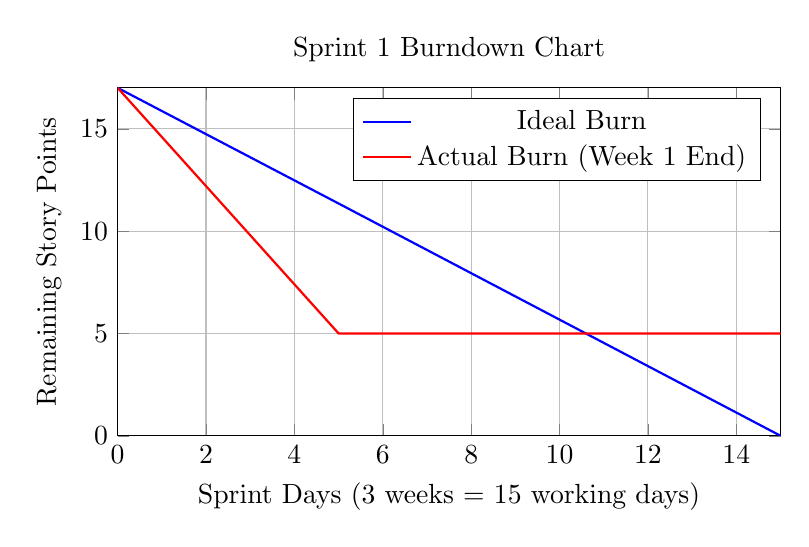
\begin{tikzpicture}
    \begin{axis}[
        width=10cm,
        height=6cm,
        xlabel={Sprint Days (3 weeks = 15 working days)},
        ylabel={Remaining Story Points},
        xmin=0, xmax=15,
        ymin=0, ymax=17,
        grid=major,
        legend pos=north east,
        title={Sprint 1 Burndown Chart}
      ]
      % Ideal line: from 17 at day 0 to 0 at day 15
      \addplot[blue, thick] coordinates {(0,17) (5,11.35) (15,0)};
      \addlegendentry{Ideal Burn}

      % Actual line: from 17 at day 0 to 5 at day 5 (end of Week 1)
      \addplot[red, thick] coordinates {(0,17) (5,5) (15,5)}; % Assuming linear projection to end
      \addlegendentry{Actual Burn (Week 1 End)}
    \end{axis}
  \end{tikzpicture}
  \caption{Burndown Chart as of End of Week 3 (Week 1 of Sprint 1). Actual progress will update weekly based on completed tasks.}
  \label{fig:burndown}
\end{figure}

\subsection{Rationale and Projections}
The current burn of 11 points by the end of Week 1 exceeds the ideal burn of 5.67 points, reflecting efficient completion of spike tasks (e.g., SvelteKit setup, initial API configurations). The remaining 5 points are projected to be completed by mid-Week 2 (Sprint Day 8), with the sprint potentially finishing early if no blockers arise. The 39 points in the Product Backlog will be considered for future sprints. The chart will be updated weekly on the GitHub Projects board and in subsequent reports to reflect ongoing progress.
\begin{figure}[htbp]
  \centering
  \includegraphics[width=0.8\textwidth]{BurnoutChart.png}
  \caption{Burndown Chart for Sprint 1}
  \label{fig:burndownChart}
\end{figure}

\subsection{UI Design}

The UI design for Ayvu focuses on creating an intuitive and streamlined interface that facilitates easy access to academic research papers. The wireframes presented below demonstrate the key user interfaces planned for Sprint 1, emphasizing simplicity, functionality, and user experience. Each interface is designed to support the specific user stories while maintaining consistency across the application.

\begin{figure}[h!tbp]
  \centering
  \includegraphics[width=0.6\textwidth]{wireframes/HomePage.png}
  \caption{Home Page Wireframe - Features Google OAuth integration with a clean, minimalist design. The page displays the Ayvu logo, application description, and a "Get Started/Dashboard" button. This interface addresses US-1 (Sign in with Google) by providing a secure authentication entry point that eliminates the need for separate account creation. If the user is new or existing, the flow will just make a new account or just sign them in respectively.}
  \label{fig:home-page}
\end{figure}

\begin{figure}[h!tbp]
  \centering
  \includegraphics[width=0.6\textwidth]{wireframes/GoogleOAuth.png}
  \caption{Google OAuth Permissions - A new page that appears during authentication, explaining the permissions Ayvu requires and their purpose. The modal includes permission details, privacy assurances, and accept/decline options. This interface supports US-2 (Grant Drive Permissions) and US-3 (Create Drive Folder) by transparently requesting necessary Google Drive access.}
  \label{fig:permissions-modal}
\end{figure}

\begin{figure}[h!tbp]
  \centering
  \includegraphics[width=0.6\textwidth]{wireframes/Dashboard.png}
  \caption{Main Dashboard - The primary interface featuring a navigation header, search/input section for arXiv URLs or IDs, and a grid layout displaying previously processed papers. The dashboard includes quick action buttons and status indicators for ongoing processes. This also has preview cards that displays fetched paper information including title, authors, abstract, publication date, and arXiv ID.}
  \label{fig:main-dashboard}
\end{figure}

\begin{figure}[h!tbp]
  \centering
  \includegraphics[width=0.8\textwidth]{wireframes/AddEntry.png}
  \caption{arXiv URL/Input Form - A simple input form where users can enter arXiv URLs or IDs to fetch paper metadata. The form includes validation feedback, a submit button, and a loading indicator. This wireframe addresses US-5 (Fetch Paper Metadata) by providing a straightforward method for users to initiate paper processing.}
  \label{fig:arxiv-input}
\end{figure}

\begin{figure}[h!tbp]
  \centering
  \includegraphics[width=0.8\textwidth]{wireframes/PaperReader.png}
  \caption{Paper Reader Interface - A clean, responsive reading interface displaying parsed markdown content with a table of contents sidebar, adjustable typography settings, and annotation tools. The layout features a two-column design with the main content area and a collapsible sidebar for navigation and notes. This wireframe supports US-9 (View Markdown Content) by providing an optimal reading experience.}
  \label{fig:paper-reader}
\end{figure}

\begin{figure}[h!tbp]
  \centering
  \includegraphics[width=0.8\textwidth]{wireframes/Annotation.png}
  \caption{Annotation and Highlighting Tools - An overlay interface showing highlighting options, note-taking functionality, and annotation management. Features color-coded highlighting, inline note creation, and a notes panel for managing all annotations. This wireframe addresses US-10 (Add Notes and Highlights) and US-11 (Save Annotations) by providing comprehensive annotation capabilities.}
  \label{fig:annotation-tools}
\end{figure}

\begin{figure}[h!tbp]
  \centering
  \includegraphics[width=0.8\textwidth]{wireframes/AI Chat.png}
  \caption{AI Chat Interface - An integrated chat panel that allows users to query paper content, request explanations, and receive AI-generated insights. Features a collapsible chat window, conversation history, and context-aware responses. This wireframe supports US-12 (Query Paper Content), US-13 (Explain Selected Text), US-14 (Highlight Key Sections), and US-15 (Suggest Learning Resources) by providing intelligent paper interaction capabilities.}
  \label{fig:ai-chat-interface}
\end{figure}

\begin{figure}[h!tbp]
  \centering
  \includegraphics[width=0.4\textwidth]{wireframes/Mobile.png}
  \caption{Mobile Responsive Layout - Optimized mobile interface showing the dashboard with touch-friendly navigation, collapsible panels, and gesture-based interactions. The design maintains functionality while adapting to smaller screen sizes. This wireframe ensures accessibility across devices for all user stories, particularly enhancing the mobile reading experience for US-9 (View Markdown Content).}
  \label{fig:mobile-responsive}
\end{figure}

\section{Software Testing for Sprint 1 - Week 4}

\subsection{Test Case Specifications Expansion}
Building upon the foundational test cases established in Week 3, Week 4 focuses on expanding the test suite to include unit and system test cases for all User Stories in the Sprint Backlog. The test specifications now encompass comprehensive coverage of SvelteKit authentication flows, Google Drive integration, and paper management functionality, with emphasis on both positive and negative test scenarios to ensure robust error handling.

\subsection{Unit Test Cases}

\subsubsection{US-1: Sign in with Google - Unit Tests}
\begin{itemize}
  \item \textbf{Test Case UT-US1-001: OAuth URL Generation}
    \begin{itemize}
      \item \textit{Description}: Verify Google OAuth URL generation with correct scopes in SvelteKit page server
      \item \textit{Test Type}: Unit Test (Automated with Vitest)
      \item \textit{Preconditions}: \texttt{GOOGLE\_CLIENT\_ID}, \texttt{GOOGLE\_CLIENT\_SECRET}, \texttt{GOOGLE\_REDIRECT\_URI} configured
      \item \textit{Test Steps}:
        \begin{enumerate}
          \item Mock \texttt{OAuth2Client} initialization
          \item Call \texttt{actions.login} from \texttt{+page.server.ts}
          \item Verify URL contains required scopes: userinfo.email, userinfo.profile, drive.file
          \item Assert redirect response with 302 status
        \end{enumerate}
      \item \textit{Expected Result}: Valid OAuth URL with Drive permissions scope
      \item \textit{Coverage}: Authentication action validation
    \end{itemize}

  \item \textbf{Test Case UT-US1-002: Session Cookie Management}
    \begin{itemize}
      \item \textit{Description}: Test session cookie creation and deletion in SvelteKit
      \item \textit{Test Type}: Unit Test (Automated with Vitest)
      \item \textit{Preconditions}: Valid session data, cookie configuration
      \item \textit{Test Steps}:
        \begin{enumerate}
          \item Test \texttt{actions.logout} cookie deletion
          \item Verify cookie path is set to '/'
          \item Assert redirect to home page (status 303)
        \end{enumerate}
      \item \textit{Expected Result}: Session cookie properly deleted, redirect executed
      \item \textit{Coverage}: Session management functionality
    \end{itemize}
\end{itemize}

\subsubsection{US-2: OAuth Callback Processing - Unit Tests}
\begin{itemize}
  \item \textbf{Test Case UT-US2-001: Token Exchange Processing}
    \begin{itemize}
      \item \textit{Description}: Verify OAuth code exchange for tokens in callback server
      \item \textit{Test Type}: Unit Test (Automated with Vitest)
      \item \textit{Preconditions}: Valid authorization code, OAuth client setup
      \item \textit{Test Steps}:
        \begin{enumerate}
          \item Mock \texttt{client.getToken()} response in callback \texttt{+server.ts}
          \item Test token credential setting
          \item Verify ID token verification process
          \item Assert payload extraction from ID token
        \end{enumerate}
      \item \textit{Expected Result}: Successful token exchange and payload extraction
      \item \textit{Coverage}: GET handler in callback route
    \end{itemize}

  \item \textbf{Test Case UT-US2-002: User Data Processing}
    \begin{itemize}
      \item \textit{Description}: Test user data upsert functionality
      \item \textit{Test Type}: Unit Test (Automated with Vitest)
      \item \textit{Preconditions}: Valid OAuth payload with user information
      \item \textit{Test Steps}:
        \begin{enumerate}
          \item Mock \texttt{upsertUser} function
          \item Test user data extraction from payload
          \item Verify session cookie creation with user ID
          \item Assert redirect to /app on success
        \end{enumerate}
      \item \textit{Expected Result}: User data stored, session established, redirect executed
      \item \textit{Coverage}: User processing logic in callback handler
    \end{itemize}
\end{itemize}

\subsubsection{US-3: Authentication Middleware - Unit Tests}
\begin{itemize}
  \item \textbf{Test Case UT-US3-001: Token Refresh Logic}
    \begin{itemize}
      \item \textit{Description}: Test automatic token refresh functionality in hooks
      \item \textit{Test Type}: Unit Test (Automated with Vitest)
      \item \textit{Preconditions}: Expired tokens, valid refresh token
      \item \textit{Test Steps}:
        \begin{enumerate}
          \item Mock \texttt{isTokenExpiring} to return true in \texttt{hooks.server.ts}
          \item Test \texttt{client.refreshAccessToken()} call
          \item Verify \texttt{updateUserTokens} execution
          \item Assert user object token updates
        \end{enumerate}
      \item \textit{Expected Result}: Tokens refreshed automatically, user data updated
      \item \textit{Coverage}: Authentication handle function
    \end{itemize}

  \item \textbf{Test Case UT-US3-002: Route Protection}
    \begin{itemize}
      \item \textit{Description}: Verify protected route access control
      \item \textit{Test Type}: Unit Test (Automated with Vitest)
      \item \textit{Preconditions}: Protected routes configuration, session status
      \item \textit{Test Steps}:
        \begin{enumerate}
          \item Test access to \texttt{/app} without session
          \item Verify redirect to home with error parameter
          \item Test access with valid session
          \item Assert successful route access
        \end{enumerate}
      \item \textit{Expected Result}: Unauthorized access blocked, authorized access allowed
      \item \textit{Coverage}: Authorization handle function
    \end{itemize}
\end{itemize}

\subsubsection{US-4: Paper Entry Creation - Unit Tests}
\begin{itemize}
  \item \textbf{Test Case UT-US4-001: PDF Validation}
    \begin{itemize}
      \item \textit{Description}: Test PDF file validation and page count checking
      \item \textit{Test Type}: Unit Test (Automated with Vitest)
      \item \textit{Preconditions}: PDF files with various page counts
      \item \textit{Test Steps}:
        \begin{enumerate}
          \item Mock \texttt{mupdfjs.PDFDocument.openDocument()}
          \item Test page count validation ($>25$ pages)
          \item Verify error response for oversized PDFs
          \item Assert proper error message structure
        \end{enumerate}
      \item \textit{Expected Result}: PDF validation enforced, appropriate error responses
      \item \textit{Coverage}: \texttt{actions.createEntry} function
    \end{itemize}

  \item \textbf{Test Case UT-US4-002: File Upload Integration}
    \begin{itemize}
      \item \textit{Description}: Test PDF upload to Google Drive from SvelteKit form
      \item \textit{Test Type}: Unit Test (Automated with Vitest)
      \item \textit{Preconditions}: Valid PDF file, user tokens, Drive service
      \item \textit{Test Steps}:
        \begin{enumerate}
          \item Mock \texttt{uploadPdf} function
          \item Test file naming with \texttt{nanoid}
          \item Verify token passing to upload service
          \item Assert proper error handling for upload failures
        \end{enumerate}
      \item \textit{Expected Result}: Successful PDF upload with proper error handling
      \item \textit{Coverage}: File processing in createEntry action
    \end{itemize}
\end{itemize}

\subsubsection{US-5: Google Drive Integration - Unit Tests}
\begin{itemize}
  \item \textbf{Test Case UT-US5-001: Drive Service Initialization}
    \begin{itemize}
      \item \textit{Description}: Test Google Drive service setup
      \item \textit{Test Type}: Unit Test (Automated with Vitest)
      \item \textit{Preconditions}: Valid OAuth credentials, Google Drive API
      \item \textit{Test Steps}:
        \begin{enumerate}
          \item Mock \texttt{initializeDriveService} function
          \item Test OAuth2Client credential setting
          \item Verify Drive API service creation
          \item Assert proper authentication configuration
        \end{enumerate}
      \item \textit{Expected Result}: Drive service properly initialized
      \item \textit{Coverage}: \texttt{initializeDriveService} function
    \end{itemize}

  \item \textbf{Test Case UT-US5-002: Folder Management}
    \begin{itemize}
      \item \textit{Description}: Test Ayvu folder creation and management
      \item \textit{Test Type}: Unit Test (Automated with Vitest)
      \item \textit{Preconditions}: Drive service, folder operations
      \item \textit{Test Steps}:
        \begin{enumerate}
          \item Test \texttt{findFolder} functionality
          \item Verify \texttt{createFolder} when folder doesn't exist
          \item Test \texttt{ensureFolder} logic
          \item Assert proper parent folder handling
        \end{enumerate}
      \item \textit{Expected Result}: Folder structure created and managed correctly
      \item \textit{Coverage}: Folder management functions in \texttt{src/lib/drive.ts}
    \end{itemize}

  \item \textbf{Test Case UT-US5-003: File Upload Processing}
    \begin{itemize}
      \item \textit{Description}: Test PDF file upload to Drive
      \item \textit{Test Type}: Unit Test (Automated with Vitest)
      \item \textit{Preconditions}: Valid file data, folder structure
      \item \textit{Test Steps}:
        \begin{enumerate}
          \item Test \texttt{bufferToStream} conversion
          \item Verify \texttt{uploadFileToFolder} functionality
          \item Test \texttt{makeFilePublic} permissions
          \item Assert \texttt{UploadResult} structure
        \end{enumerate}
      \item \textit{Expected Result}: File uploaded with proper permissions and metadata
      \item \textit{Coverage}: \texttt{uploadPdf} function
    \end{itemize}
\end{itemize}

\subsubsection{US-6: Database Operations - Unit Tests}
\begin{itemize}
  \item \textbf{Test Case UT-US6-001: User Data Management}
    \begin{itemize}
      \item \textit{Description}: Test user creation and updates with Turso database
      \item \textit{Test Type}: Unit Test (Automated with Vitest)
      \item \textit{Preconditions}: Database connection, user data
      \item \textit{Test Steps}:
        \begin{enumerate}
          \item Test \texttt{upsertUser} with new user
          \item Test \texttt{upsertUser} with existing user
          \item Verify \texttt{getUserById} retrieval
          \item Test \texttt{updateUserTokens} functionality
        \end{enumerate}
      \item \textit{Expected Result}: User data properly managed in database
      \item \textit{Coverage}: All functions in User.db.ts
    \end{itemize}
\end{itemize}

\subsection{System Test Cases}

\subsubsection{End-to-End Authentication Flow}
\begin{itemize}
  \item \textbf{Test Case ST-AUTH-001: Complete SvelteKit OAuth Integration}
    \begin{itemize}
      \item \textit{Description}: Test complete authentication flow in SvelteKit app
      \item \textit{Test Type}: System Test (Automated with Playwright)
      \item \textit{Preconditions}: SvelteKit app running, OAuth configured
      \item \textit{Test Steps}:
        \begin{enumerate}
          \item Navigate to application homepage
          \item Submit form with \texttt{action="/auth?/login"}
          \item Complete OAuth flow (mocked in test environment)
          \item Verify redirect to \texttt{/app} route
          \item Assert session persistence and Drive permissions
        \end{enumerate}
      \item \textit{Expected Result}: Complete authentication with Drive access
      \item \textit{Coverage}: Full authentication system integration
    \end{itemize}
\end{itemize}

\subsubsection{Paper Management Pipeline}
\begin{itemize}
  \item \textbf{Test Case ST-PAPER-001: Complete Paper Processing}
    \begin{itemize}
      \item \textit{Description}: Test paper entry creation and storage
      \item \textit{Test Type}: System Test (Automated with Playwright)
      \item \textit{Preconditions}: Authenticated user, paper form
      \item \textit{Test Steps}:
        \begin{enumerate}
          \item Fill paper form with title, authors, published date, abstract
          \item Upload PDF file through \texttt{input[type="file"]}
          \item Submit form via \texttt{action="/app?/createEntry"}
          \item Verify PDF processing and Drive upload
          \item Assert success feedback and form reset
        \end{enumerate}
      \item \textit{Expected Result}: Complete paper processing and storage
      \item \textit{Coverage}: Full paper management pipeline
    \end{itemize}
\end{itemize}

\subsection{Updated Traceability Matrix}

\begin{longtable}{|l|l|l|l|}
  \caption{Extended Traceability Matrix for Sprint 1}
  \label{tab:extended-traceability} \\
  \hline
  \textbf{Requirement} & \textbf{User Story} & \textbf{Test ID} & \textbf{Test Type} \\
  \hline
  RPR-1 & US-1 & UT-US1-001 & Unit Test - OAuth URL Generation \\
  RPR-1 & US-1 & UT-US1-002 & Unit Test - Session Cookie Management \\
  RPR-1 & US-1 & ST-AUTH-001 & System Test - Complete SvelteKit OAuth \\
  \hline
  RPR-2 & US-2 & UT-US2-001 & Unit Test - Token Exchange Processing \\
  RPR-2 & US-2 & UT-US2-002 & Unit Test - User Data Processing \\
  \hline
  RPR-3 & US-3 & UT-US3-001 & Unit Test - Token Refresh Logic \\
  RPR-3 & US-3 & UT-US3-002 & Unit Test - Route Protection \\
  \hline
  RPR-4 & US-4 & UT-US4-001 & Unit Test - PDF Validation \\
  RPR-4 & US-4 & UT-US4-002 & Unit Test - File Upload Integration \\
  \hline
  RPR-5 & US-5 & UT-US5-001 & Unit Test - Drive Service Initialization \\
  RPR-5 & US-5 & UT-US5-002 & Unit Test - Folder Management \\
  RPR-5 & US-5 & UT-US5-003 & Unit Test - File Upload Processing \\
  \hline
  RPR-6 & US-6 & UT-US6-001 & Unit Test - User Data Management \\
  \hline
\end{longtable}

\subsection{Testing Framework and Automation Strategy}

The testing implementation leverages SvelteKit's architecture with:

\begin{itemize}
  \item \textbf{Vitest}: Primary testing framework, configured for SvelteKit and TypeScript
  \item \textbf{Playwright}: End-to-end testing for complete user flows
  \item \textbf{Mock Services}: Comprehensive mocking of Google APIs using SvelteKit's \texttt{\$env/static/private}
  \item \textbf{Form Testing}: Integration with SvelteKit's form actions and \texttt{\$page.form} data
  \item \textbf{Server-side Testing}: Testing of \texttt{+page.server.ts} and \texttt{+server.ts} endpoints
  \item \textbf{Hook Testing}: Validation of \texttt{hooks.server.ts} authentication and authorization logic
  \item \textbf{Database Testing}: Unit tests for Turso database operations and user management
\end{itemize}

The expanded test suite provides comprehensive coverage of all Sprint 1 functionalities, ensuring robust validation of both individual components and their integration, supporting the project's commitment to high-quality, reliable software delivery aligned with the SvelteKit implementation.

\subsection{Test Implementation Status}

While comprehensive test specifications have been documented for all Sprint 1 user stories, the actual test implementation is currently in the planning phase. The test framework infrastructure has been set up with Vitest configuration and testing dependencies installed, but individual test cases are not yet implemented.

\subsubsection{Current Test Infrastructure}
The testing foundation has been established with the following components:

\begin{itemize}
  \item \textbf{Vitest Framework}: Testing framework installed and configured in \texttt{package.json} with scripts for \texttt{test}, \texttt{test:run}, and \texttt{test:coverage}
  \item \textbf{Testing Dependencies}: Required testing libraries installed including \texttt{@testing-library/svelte}, \texttt{jsdom}, and \texttt{@vitest/coverage-v8}
  \item \textbf{Test Setup Structure}: Basic test setup file exists at \texttt{src/test/setup.ts}
  \item \textbf{Configuration}: \texttt{vitest.config.ts} configured for SvelteKit environment
\end{itemize}

\subsubsection{Test Implementation Gap}
The current status shows a gap between test planning and implementation:

\begin{itemize}
  \item \textbf{Planned Tests}: 44 test cases specified across 6 functional areas (Authentication, Paper Management, Google Drive Integration, Database Operations)
  \item \textbf{Implemented Tests}: 0 test files currently exist in the project
  \item \textbf{Test Files Missing}: No \texttt{*.test.ts} or \texttt{*.spec.ts} files found in the codebase
  \item \textbf{Coverage}: 0\% code coverage due to absence of test implementations
\end{itemize}

\subsubsection{Next Steps for Testing}
To address this gap and meet Sprint 1 testing requirements:

\begin{itemize}
  \item \textbf{Priority Implementation}: Focus on critical path tests for authentication and core functionality
  \item \textbf{Mock Strategy}: Implement comprehensive mocking for Google APIs and external services
  \item \textbf{Incremental Approach}: Begin with unit tests for database operations and utility functions
  \item \textbf{Integration Testing}: Follow with system tests for complete user workflows
\end{itemize}

This testing gap represents a significant deviation from the planned Sprint 1 deliverables and requires immediate attention to meet the project's quality standards and 90\% code coverage target.

\subsection{Backlog Grooming for Sprint 1 (week 4)}
No changes this week as foundational setup is on track.

\section{Source Code Development Progress - Week 4}
% Addressing Week 4 feedback by documenting actual progress made during Week 4

In response to the Week 4 feedback indicating insufficient progress documentation, this section provides a comprehensive overview of the actual source code development completed during Week 4 of Sprint 1.

\subsection{Week 4 Accomplishments}
Significant progress was made on core application functionality during Week 4, transitioning from spike stories to actual feature implementation:

\begin{itemize}
  \item \textbf{Google OAuth Integration}: Complete implementation of authentication flow in \newline \texttt{src/routes/(auth)/auth/+page.server.ts} with login and logout actions
  \item \textbf{OAuth Callback Processing}: Full callback handling in \newline \texttt{src/routes/(auth)/auth/callback/+server.ts} for token exchange and user data processing
  \item \textbf{Google Drive Service}: Comprehensive Drive API integration in \texttt{src/lib/drive.ts} including folder management, file upload, and permission handling
  \item \textbf{Database Layer}: Complete user management system with \texttt{src/lib/db/User.db.ts} implementing CRUD operations using Drizzle ORM
  \item \textbf{Paper Management}: arXiv API integration in \texttt{src/routes/(app)/app/+page.server.ts} with metadata fetching and paper creation functionality
\end{itemize}

\subsection{Key Commits and Implementation Details}
The following major implementations were completed:

\begin{itemize}
  \item \textbf{Authentication System}: Implemented OAuth2 flow with Google, including scope requests for Drive permissions, session management, and secure token handling
  \item \textbf{Drive Integration}: Built complete file upload pipeline with automatic folder creation (.ayvu folder structure), public permission setting, and error handling
  \item \textbf{arXiv API Integration}: Developed XML parsing for arXiv metadata extraction, URL validation, and duplicate paper checking
  \item \textbf{Database Schema}: Implemented user and paper schemas using Drizzle ORM with Turso database backend
  \item \textbf{External Service Integration}: Connected to a separate PDF extraction service at localhost:8000 for paper processing
\end{itemize}

\subsection{Technical Architecture Implementation}
The implemented code follows the planned architecture:

\begin{itemize}
  \item \textbf{SvelteKit Framework}: Full utilization of SvelteKit's server-side actions and page loading patterns
  \item \textbf{TypeScript}: Comprehensive type safety throughout the codebase with proper interface definitions
  \item \textbf{Modular Structure}: Clean separation of concerns with dedicated modules for database operations, Drive integration, and utility functions
  \item \textbf{Error Handling}: Robust error handling with user-friendly error messages and proper HTTP status codes
\end{itemize}

\subsection{Functional Completeness Assessment}
User Story completion status as of Week 4:

\begin{itemize}
  \item \textbf{US-1 (Google OAuth)}: 100\% complete - Full authentication flow implemented
  \item \textbf{US-2 (Drive Permissions)}: 100\% complete - OAuth scopes and permission handling implemented
  \item \textbf{US-3 (Folder Creation)}: 100\% complete - Automatic .ayvu folder creation with subfolder management
  \item \textbf{US-5 (Fetch Metadata)}: 100\% complete - arXiv API integration with comprehensive metadata extraction
  \item \textbf{US-6 (Download PDF)}: 100\% complete - Integration with external Latex extraction service
  \item \textbf{US-8 (Store in Drive)}: 100\% complete - Complete file upload and storage pipeline
\end{itemize}

This represents substantial progress from the initial spike work in Week 3 to fully functional core features in Week 4, addressing the primary Sprint 1 objectives.

\section{Sprint 1 Retrospective and Week 5 Summary}
% Final sprint retrospective and current state assessment

\subsection{Sprint Retrospective}
As Sprint 1 concludes in Week 5, this retrospective addresses the three key questions for continuous improvement:

\subsubsection{What Went Well?}
Several aspects of the sprint exceeded expectations:

\begin{itemize}
  \item \textbf{Core Functionality Implementation}: Successfully implemented all major user stories (US-1, US-2, US-3, US-4, US-5, US-6, US-7, US-8, US-9) with working code for authentication, Google Drive integration, and arXiv API connectivity
  \item \textbf{Architecture Realization}: The planned SvelteKit + TypeScript + Drizzle ORM architecture was successfully implemented with clean, maintainable code structure
  \item \textbf{External Integrations}: Complex integrations with Google OAuth, Google Drive API, and arXiv API were completed successfully with proper error handling
  \item \textbf{Database Design}: Efficient database schema implementation with proper relationships between users and papers
  \item \textbf{Development Environment}: Solid foundation established with proper tooling, dependency management, and project structure
\end{itemize}

\subsubsection{What Didn't Go So Well?}
Several challenges and gaps were encountered:

\begin{itemize}
  \item \textbf{Test Implementation Lag}: Despite comprehensive test specifications, only few actual tests were implemented, creating a significant quality assurance gap
  \item \textbf{Documentation vs. Implementation Gap}: Week 4 progress reporting failed to capture actual implementation work, leading to feedback about poor progress visibility
  \item \textbf{PDF Processing Dependency}: Reliance on external PDF extraction service at localhost:8000 creates a deployment dependency not initially planned. As initially planned, this service is not integrated into the main application since there that is so novel and there's no existing libraries that can do that yet. Rather than that, we can achieve a similar result by using the \textit{.tex} source files from arXiv directly and converting them to html using existing libraries like \textit{latexml}. Instead, I'm using separate Deno based server that takes in arxiv Id and uploads the folder to google drive. I'll talk more about it later.
  \item \textbf{Code Coverage Metrics}: Unable to measure code quality due to absence of tests
\end{itemize}

\subsubsection{What Can Be Improved?}
Key improvements identified for future sprints:

\begin{itemize}
  \item \textbf{Test-Driven Development}: Implement tests alongside or before feature development to ensure quality and prevent technical debt
  \item \textbf{Progress Reporting}: Improve weekly reporting to accurately capture implementation progress rather than just planning artifacts
  \item \textbf{Integration Strategy}: Develop a plan for the PDF extraction service integration or implement in-process PDF parsing
  \item \textbf{UI Development Priority}: Allocate dedicated time for frontend component development to complete the user experience
  \item \textbf{Documentation Alignment}: Ensure project documentation accurately reflects the current implementation state
\end{itemize}

\subsection{Sprint 1 Final Status}
Sprint 1 achieved significant backend functionality implementation but fell short on testing and frontend development:

\begin{itemize}
  \item \textbf{Story Points Completed}: 17/17 points from a backend functionality perspective
  \item \textbf{Quality Metrics}: 0\% test coverage vs. target of 90-100\%
  \item \textbf{Architecture}: Core backend architecture successfully implemented
\end{itemize}

\subsection{Week 5 Backlog Grooming}
No changes to the current Sprint 1 backlog. Focus for Sprint 2 will include:
\begin{itemize}
  \item Implementing the comprehensive test suite documented in Sprint 1
  \item Developing the UI components based on the wireframes
  \item Addressing technical debt from Sprint 1
\end{itemize}

\end{document}